\chapter{Result}


\begin{figure}[h]
 \begin{center}
  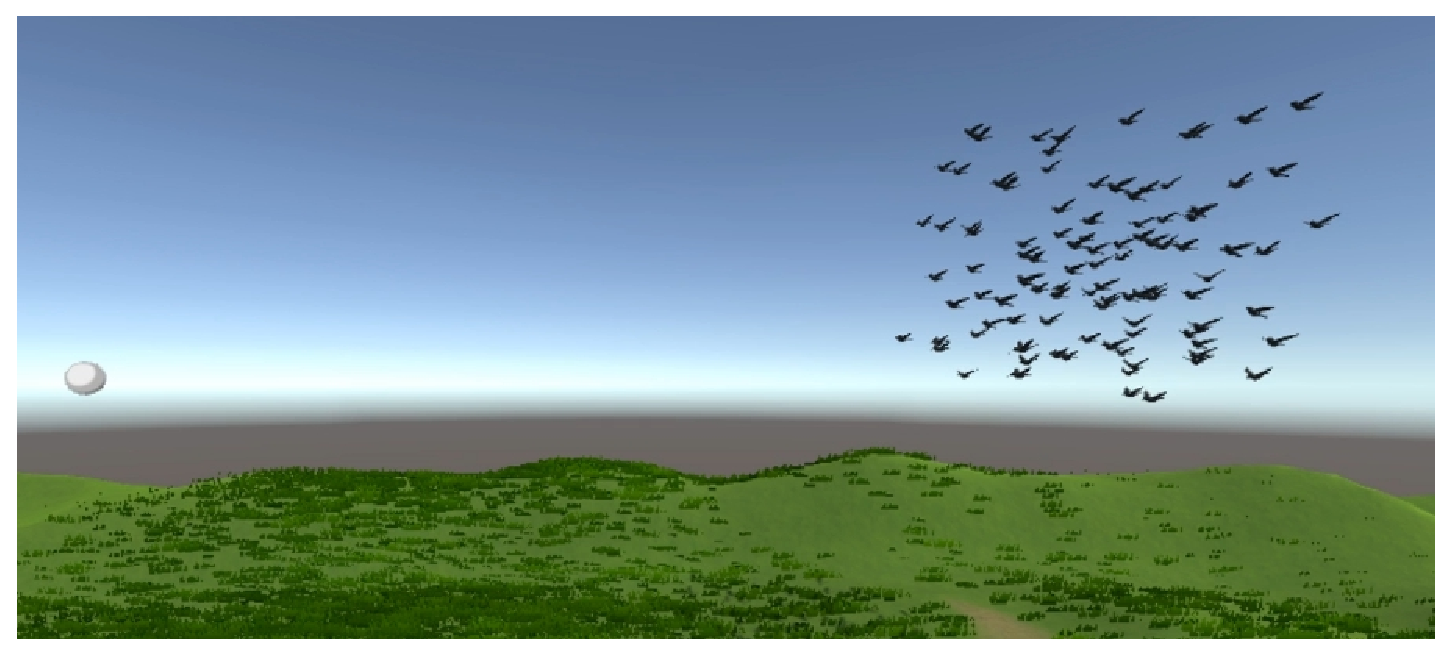
\includegraphics[width=1.0\textwidth]{simulation.eps}
 \end{center}
 \caption{A view of our flock simulation system.}
 \label{figure:simulation}
\end{figure}


Due to difficulties of obtaining real bird video, we implemented a bird flock simulation system and capture the flock motion as input video to test our system. The simulation system is based on boid model, which assumes a flock is simply the result of the interaction between the behaviors of individual birds. With these behaviors, the system can produce fine flock motion with numbers of birds. However, boid model can only model flock wandering behavior. That is, after assigning initial parameters, all birds become uncontrollable during the simulation, and the simulation always produces same results. To keep the diversity of the generated simulation result, we further include the homing behavior introduced in \cite{Shape,OB1}. With this behavior, we can generate different flock motions efficiently. After the simulation result is generated, we capture videos from it in various angles. Figure \ref{figure:simulation} shows a view of our flock simulation system. The videos are then used as inputs to our system.


\begin{figure}[h]
 \begin{center}
  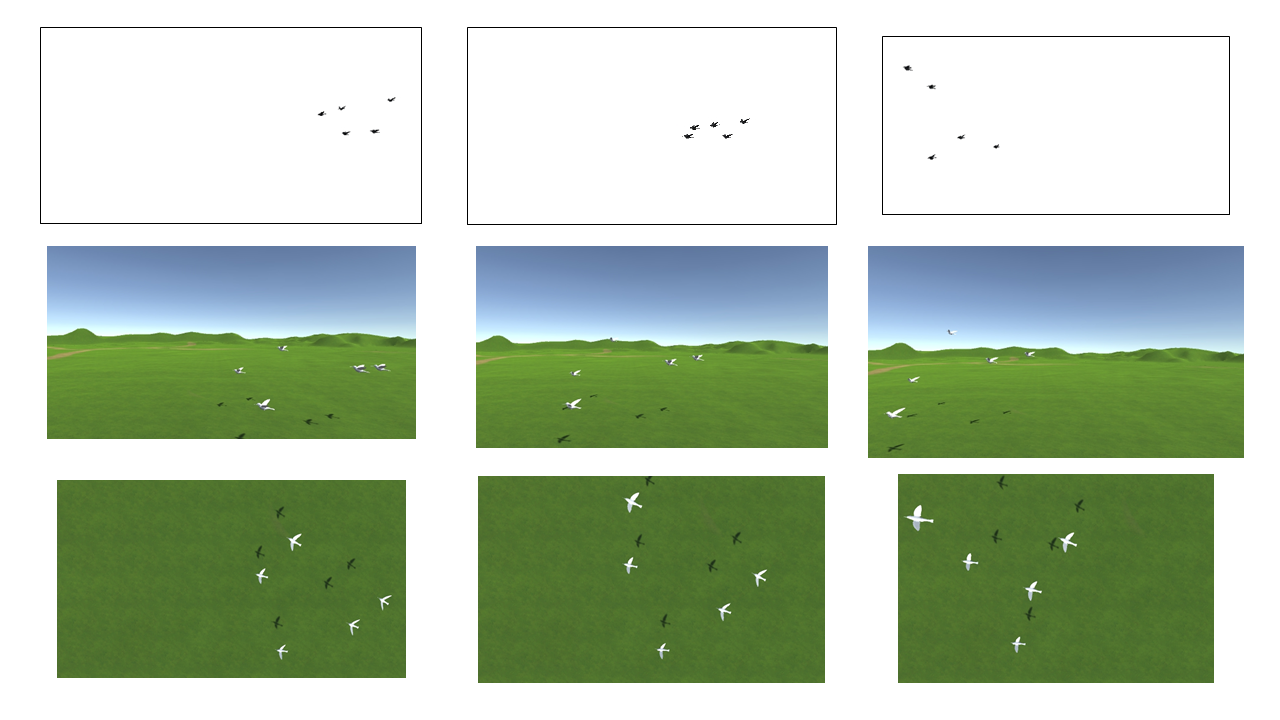
\includegraphics[width=1.0\textwidth]{result1.eps}
 \end{center}
 \caption{Result1:(top)input video. (middle)generated result from side view. (bottom)generated result from top view.}
 \label{figure:result1_side}
\end{figure}


We have tested several video inputs generated from flock simulation system. In figure \ref{figure:result1}, the generated flock motion contains 5 birds with 200-frames.


(TODO: MORE RESULT)
